% Options for packages loaded elsewhere
\PassOptionsToPackage{unicode}{hyperref}
\PassOptionsToPackage{hyphens}{url}
%
\documentclass[
]{article}
\usepackage{lmodern}
\usepackage{amssymb,amsmath}
\usepackage{ifxetex,ifluatex}
\ifnum 0\ifxetex 1\fi\ifluatex 1\fi=0 % if pdftex
  \usepackage[T1]{fontenc}
  \usepackage[utf8]{inputenc}
  \usepackage{textcomp} % provide euro and other symbols
\else % if luatex or xetex
  \usepackage{unicode-math}
  \defaultfontfeatures{Scale=MatchLowercase}
  \defaultfontfeatures[\rmfamily]{Ligatures=TeX,Scale=1}
\fi
% Use upquote if available, for straight quotes in verbatim environments
\IfFileExists{upquote.sty}{\usepackage{upquote}}{}
\IfFileExists{microtype.sty}{% use microtype if available
  \usepackage[]{microtype}
  \UseMicrotypeSet[protrusion]{basicmath} % disable protrusion for tt fonts
}{}
\makeatletter
\@ifundefined{KOMAClassName}{% if non-KOMA class
  \IfFileExists{parskip.sty}{%
    \usepackage{parskip}
  }{% else
    \setlength{\parindent}{0pt}
    \setlength{\parskip}{6pt plus 2pt minus 1pt}}
}{% if KOMA class
  \KOMAoptions{parskip=half}}
\makeatother
\usepackage{xcolor}
\IfFileExists{xurl.sty}{\usepackage{xurl}}{} % add URL line breaks if available
\IfFileExists{bookmark.sty}{\usepackage{bookmark}}{\usepackage{hyperref}}
\hypersetup{
  pdftitle={Survival Analysis of Post-Myocardial Infarction Patients},
  pdfauthor={Alvein, Orr, Pham},
  hidelinks,
  pdfcreator={LaTeX via pandoc}}
\urlstyle{same} % disable monospaced font for URLs
\usepackage[margin=1in]{geometry}
\usepackage{color}
\usepackage{fancyvrb}
\newcommand{\VerbBar}{|}
\newcommand{\VERB}{\Verb[commandchars=\\\{\}]}
\DefineVerbatimEnvironment{Highlighting}{Verbatim}{commandchars=\\\{\}}
% Add ',fontsize=\small' for more characters per line
\usepackage{framed}
\definecolor{shadecolor}{RGB}{248,248,248}
\newenvironment{Shaded}{\begin{snugshade}}{\end{snugshade}}
\newcommand{\AlertTok}[1]{\textcolor[rgb]{0.94,0.16,0.16}{#1}}
\newcommand{\AnnotationTok}[1]{\textcolor[rgb]{0.56,0.35,0.01}{\textbf{\textit{#1}}}}
\newcommand{\AttributeTok}[1]{\textcolor[rgb]{0.77,0.63,0.00}{#1}}
\newcommand{\BaseNTok}[1]{\textcolor[rgb]{0.00,0.00,0.81}{#1}}
\newcommand{\BuiltInTok}[1]{#1}
\newcommand{\CharTok}[1]{\textcolor[rgb]{0.31,0.60,0.02}{#1}}
\newcommand{\CommentTok}[1]{\textcolor[rgb]{0.56,0.35,0.01}{\textit{#1}}}
\newcommand{\CommentVarTok}[1]{\textcolor[rgb]{0.56,0.35,0.01}{\textbf{\textit{#1}}}}
\newcommand{\ConstantTok}[1]{\textcolor[rgb]{0.00,0.00,0.00}{#1}}
\newcommand{\ControlFlowTok}[1]{\textcolor[rgb]{0.13,0.29,0.53}{\textbf{#1}}}
\newcommand{\DataTypeTok}[1]{\textcolor[rgb]{0.13,0.29,0.53}{#1}}
\newcommand{\DecValTok}[1]{\textcolor[rgb]{0.00,0.00,0.81}{#1}}
\newcommand{\DocumentationTok}[1]{\textcolor[rgb]{0.56,0.35,0.01}{\textbf{\textit{#1}}}}
\newcommand{\ErrorTok}[1]{\textcolor[rgb]{0.64,0.00,0.00}{\textbf{#1}}}
\newcommand{\ExtensionTok}[1]{#1}
\newcommand{\FloatTok}[1]{\textcolor[rgb]{0.00,0.00,0.81}{#1}}
\newcommand{\FunctionTok}[1]{\textcolor[rgb]{0.00,0.00,0.00}{#1}}
\newcommand{\ImportTok}[1]{#1}
\newcommand{\InformationTok}[1]{\textcolor[rgb]{0.56,0.35,0.01}{\textbf{\textit{#1}}}}
\newcommand{\KeywordTok}[1]{\textcolor[rgb]{0.13,0.29,0.53}{\textbf{#1}}}
\newcommand{\NormalTok}[1]{#1}
\newcommand{\OperatorTok}[1]{\textcolor[rgb]{0.81,0.36,0.00}{\textbf{#1}}}
\newcommand{\OtherTok}[1]{\textcolor[rgb]{0.56,0.35,0.01}{#1}}
\newcommand{\PreprocessorTok}[1]{\textcolor[rgb]{0.56,0.35,0.01}{\textit{#1}}}
\newcommand{\RegionMarkerTok}[1]{#1}
\newcommand{\SpecialCharTok}[1]{\textcolor[rgb]{0.00,0.00,0.00}{#1}}
\newcommand{\SpecialStringTok}[1]{\textcolor[rgb]{0.31,0.60,0.02}{#1}}
\newcommand{\StringTok}[1]{\textcolor[rgb]{0.31,0.60,0.02}{#1}}
\newcommand{\VariableTok}[1]{\textcolor[rgb]{0.00,0.00,0.00}{#1}}
\newcommand{\VerbatimStringTok}[1]{\textcolor[rgb]{0.31,0.60,0.02}{#1}}
\newcommand{\WarningTok}[1]{\textcolor[rgb]{0.56,0.35,0.01}{\textbf{\textit{#1}}}}
\usepackage{graphicx,grffile}
\makeatletter
\def\maxwidth{\ifdim\Gin@nat@width>\linewidth\linewidth\else\Gin@nat@width\fi}
\def\maxheight{\ifdim\Gin@nat@height>\textheight\textheight\else\Gin@nat@height\fi}
\makeatother
% Scale images if necessary, so that they will not overflow the page
% margins by default, and it is still possible to overwrite the defaults
% using explicit options in \includegraphics[width, height, ...]{}
\setkeys{Gin}{width=\maxwidth,height=\maxheight,keepaspectratio}
% Set default figure placement to htbp
\makeatletter
\def\fps@figure{htbp}
\makeatother
\setlength{\emergencystretch}{3em} % prevent overfull lines
\providecommand{\tightlist}{%
  \setlength{\itemsep}{0pt}\setlength{\parskip}{0pt}}
\setcounter{secnumdepth}{-\maxdimen} % remove section numbering
\usepackage{booktabs}
\usepackage{longtable}
\usepackage{array}
\usepackage{multirow}
\usepackage{wrapfig}
\usepackage{float}
\usepackage{colortbl}
\usepackage{pdflscape}
\usepackage{tabu}
\usepackage{threeparttable}
\usepackage{threeparttablex}
\usepackage[normalem]{ulem}
\usepackage{makecell}
\usepackage{xcolor}

\title{Survival Analysis of Post-Myocardial Infarction Patients}
\author{Alvein, Orr, Pham}
\date{5/22/2020}

\begin{document}
\maketitle

\hypertarget{abstract}{%
\section{Abstract}\label{abstract}}

\hypertarget{background}{%
\subsubsection{Background}\label{background}}

The rates of myocardial infarction is becoming an increasing common
occurence in the United States. Rapid development of medical technology
and knowledge have led to an decline in myocardial infarction fatalities
(Gu, et al 1999). However, there is much to be learned regarding the
survival probabilities of patients following an infarction episode.Some
studies have already examined the effects of externalities on the
survival rates of these patients (Rimm, et al.~1995).

\hypertarget{objectives}{%
\subsubsection{Objectives}\label{objectives}}

Our goal is to provide detailed survival statistics of patients during a
post-myocardial infarction time period with specific concern addressed
to age, ventricular activity, and physiological cardic state. Using
these variables, we aim to provide succinct information on the current
state of the dataset as well as provide robust predictors for the future
estimates of survival for future patients.

We aim to fit non-parametric (Kaplan-Meier) and parameters curves to
describe the data as well as choose a regression model to be used for
predictive surviability.

\hypertarget{methods}{%
\subsubsection{Methods}\label{methods}}

Data from 133 post-myocardial infarction patients measure the time in
months until death in a one year monitoring period of follow-up. We use
a combination of nonparametric (Kaplan-Meier) and parametric methods
(Weilbull, Log-Normal, Log-Logistic, Cox PH) to determine estimates of
survival among gender and physiological cardic state (contraction depth,
muscular activity, anatomical status). We fit multiple distributions
over the dataset to provide current-state information of the patient
dataset. Then, we regress multiple models and use combination of Akaike
Information (AIC) statistics, logistic ratio tests, and residual
analysis to determine model adequacy.

\hypertarget{results}{%
\subsubsection{Results}\label{results}}

Initial non-parametric Kaplan-Meier curve shows a median survival time
of \textasciitilde30 months for all age groups. We choose a Weibull
regression fit (tenative) for predictive model as we have favorable AIC,
ratio, and residual indicators out of all of our model.

\hypertarget{conclusion}{%
\subsubsection{Conclusion}\label{conclusion}}

Thus, for predictive model we found the Weibull regression fit to be the
most ideal candidate for modeling survivability for patient groups.
Additionally, when examining the survival times for the Kaplan-Meier
step curve, we see that the younger age groups do survive as well as
their older counterparts. Given our limited sample size for that
population, we recommend continued studies into external effects of the
post-mycardial episode survival.

\hypertarget{introduction}{%
\section{Introduction}\label{introduction}}

Heart disease has become the leading cause of US deaths among all racial
and ethnic groups (Heron 2019, Fryar 2012). In 2009 cardiovascular
disease represented nearly 64\% of all cardiac related deaths (Dalen,
et. Al. 2014). These myocardial infarctions -- commonly known as heart
attacks - are becoming largely common among all U.S. demographic
populations. As such, researchers are looking to understand the
underlying causes of these episodes. Specifically, increases in
cardiovascular disease (CVD) cases have been largely attributed to many
risk factors such as high levels of low-density lipoproteins (LPL), high
blood pressure, and smoking (Fryar 2012).

These variables are often the results of lifestyle choices and effects
of poverty. The prevalence of the disease has closely been followed a
large body of conducted researchers aiming to reduce either the number
of these cases or reduce the mortality of the specific myocardial
infarction rates. Between 1980 and 2002, mortality rates saw a decrease
of approximately 49\% (Wilmot 2015). Decreases in mortality was common
through the world better medical intervention techniques and increase
awareness of healthier lifestyle choices became more prevalent (Goldman,
et al.~1984).

Unsurprisingly, as more patients survive CVD related infarction
episodes, more detail has been paid to understand the survivability the
time period following an episode. Wall motion score (a measure of heart
contractility during cycling) was significantly higher in those that
survived versus those that died (Kan, et. Al. 1986). We hope to examine
several factors that determine survivability among these patients. In
addition to wall motion score, we hope to stratify and understand the
relationships between time to event (death) measurements compared to
general heart health and age. Our goal is to describe the survivability
of our dataset and provide a model to predict the factors that determine
survability in the one-year period following a myocardial infarction
episode.

\hypertarget{dataset}{%
\section{Dataset}\label{dataset}}

Our data was obtained our data set from Kaggle via the Reed Institute.
The data set contains 133 total patient observations and records 8
variables. Two patient survival times were not given; thus, we elected
to remove those values to develop the most accurate portrayal of
survival times.

Since the time of myocardial infarction varies (depending if a patient
joined the study prior to the starat), some patients were followed for
less than a year. This provides a clear censoring and truncation
provide. We will address this specifically in the following section.

It should be noted the the dataset have 40 missing values after the
removal of the two patients. To develop estimates for the missing dated,
we employed a k-nearest Neighbor algorithmic approach to predict the
values for the missing values. With this in mind, our predictive and
summary models will have less than ideal accuracy.

The reader may find a summary of tables and original dataset in the
appendix of this paper.

\hypertarget{imputation}{%
\subsubsection{Imputation}\label{imputation}}

In addition to the two rows that we removed, we further modified the
dataset. The provided data contains 40 missing values that we chose to
impute using the random forest algorithm methods in the missForest R
package. Below is a summary of the missing data:

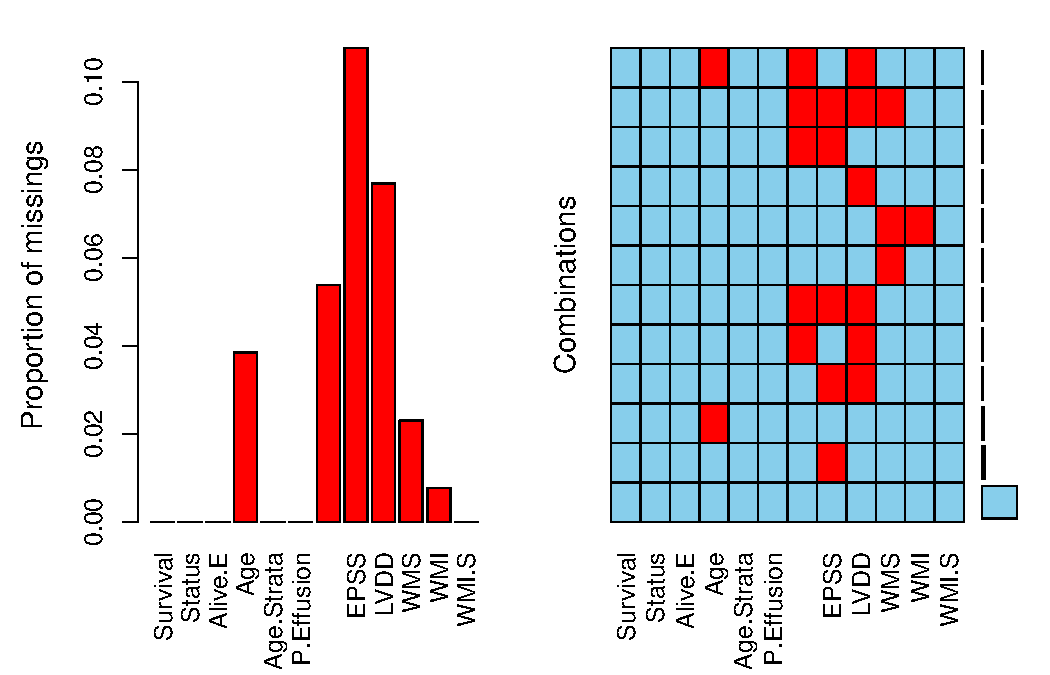
\includegraphics{markdown_files/figure-latex/missing.table-1.pdf}

\begin{table}[!h]

\caption{\label{tab:missing.table}Missing Values in Original Dataset}
\centering
\begin{tabular}[t]{l|l|r}
\hline
  & Variable & Count\\
\hline
Survival & Survival & 0\\
\hline
Status & Status & 0\\
\hline
Alive.E & Alive.E & 0\\
\hline
Age & Age & 5\\
\hline
Age.Strata & Age.Strata & 0\\
\hline
P.Effusion & P.Effusion & 0\\
\hline
F.Shortening & F.Shortening & 7\\
\hline
EPSS & EPSS & 14\\
\hline
LVDD & LVDD & 10\\
\hline
WMS & WMS & 3\\
\hline
WMI & WMI & 1\\
\hline
WMI.S & WMI.S & 0\\
\hline
\end{tabular}
\end{table}

We leverage the missForest package that uses algorithmic process used
here uses a modified k-nearest neighbot (KNN) approach. Using a training
data set, the routines of the algorithm predicts the missing values
trained on the observed parts of the dataset (Stekhoven 2012). Refer to
Stekhoven, et. al 2012 for more detail. Below is

Following imputation, we verify the imputation accuracy using the
normalized root mean squared error as an indicator of accuracy (NRMSE,
Oba et al.~(2003)). The general performance of our imputated dataset can
be expressed by:

\[ NRMSE\ =\ \sqrt{\frac{mean\left(\left(X^{true}-X^{imp}\right)^2\right)}{var\left(X^{true}\right)}} \]

Where X is a matrix of our dataset. Our calculated NRMSE is as follows:

\begin{verbatim}
##   missForest iteration 1 in progress...done!
##   missForest iteration 2 in progress...done!
##   missForest iteration 3 in progress...done!
##   missForest iteration 4 in progress...done!
\end{verbatim}

Being a random forest iterative process, each imputed dataset will be
different from each other. Out of 500 iterations, we have an averaged
NRMSE value of 0.2246 - that is our inputted values have an estimate
22.46\% deviation from estimated true accuracy.

The full imputed dataset may be found in the appendix of this paper. As
well as references to the authors who created the algorithm.

\hypertarget{censoring}{%
\subsubsection{Censoring}\label{censoring}}

Our dataset has numerous censored valued - that is, valued that cannot
be recorded due the constrainst of the study design. In our data set, we
are exmaining the survival after a heart attack, that is, the event of
interest is death given that a patient has had already survived a heart
attack (left truncation).

We have fixed start and end dates for when the data was collection. Some
patients joined when the study began. Others joined later after the
start date. Because of this, we cannot accurately determine how long a
patient survived after our observation period is over. In addition,
there are some patients that have been lost to follow up or may have
died due to the onset of other unrelated factors. These data present
themselves as being randomly right censored.

\hypertarget{methodology}{%
\section{Methodology}\label{methodology}}

Here, we brief review the methodology and theory behind our analysis
techniques for context.

\hypertarget{non-parametric-kaplan-meier}{%
\subsection{Non-Parametric: Kaplan
Meier}\label{non-parametric-kaplan-meier}}

We use Kaplan-Meier (KM) survival estimators to model a step curve for
the survival of our censored dataset. The KM estimator is an adjustment
of an empirical survival function to reflect the presence of
right-censored observations (Tableman \& Kim, 2004). The estimator can
be described in the following equation:

\[ \hat{S}(t) = \prod_{y_{(i)}\leq{t}}^{k} p_i = \prod_{i=1}^{k} (\frac{n_i -d_i}{n_i}) \]

Where \$ n\_i \$ is the number alive before time \$ y\_i \$ and \$ d\_i
\$ is the number of events during during that interval. In our case, \$
y\_i \$ is the specific patient being observed, \$ n\_i \$ is the number
of patients alive at time \$ y\_i \$. With \$ k = 131 \$, our KM
equation is:

\[ \hat{S}(t) = \prod_{i=1}^{131} (\frac{n_i -d_i}{n_i}) \]

We use this equation to estimate the survival at each time interval. We
conduct this analysis for the whole data set and then choose to stratify
on age, pericadial effusion presence, and wall motion score. We also
include cumulative hazard estimators based on the KM fit.

\hypertarget{cumulative-hazard-estimators}{%
\subsubsection{Cumulative Hazard
Estimators}\label{cumulative-hazard-estimators}}

The relationship between KM and hazard can be model by the following
equation (Tableman \& Kim, 2004):

\[ haaazzaaarrrddd\  \]

\begin{itemize}
\tightlist
\item
  define variables. Make notes
\end{itemize}

\hypertarget{parametric-estimates-log-normal-distribution}{%
\subsection{Parametric Estimates: Log-Normal
Distribution}\label{parametric-estimates-log-normal-distribution}}

\hypertarget{parametric-estimates-log-logistic-distribution}{%
\subsection{Parametric Estimates: Log-Logistic
Distribution}\label{parametric-estimates-log-logistic-distribution}}

\hypertarget{parametric-estimates-weibull-distribution}{%
\subsection{Parametric Estimates: Weibull
Distribution}\label{parametric-estimates-weibull-distribution}}

\hypertarget{hazard-estimates}{%
\subsection{Hazard Estimates}\label{hazard-estimates}}

\hypertarget{regression-model-selection}{%
\subsection{Regression \& Model
Selection}\label{regression-model-selection}}

\hypertarget{results-1}{%
\section{Results}\label{results-1}}

\hypertarget{exploratory-data-analysis}{%
\subsection{Exploratory Data Analysis}\label{exploratory-data-analysis}}

\hypertarget{non-parametric-kaplan-meier-survival-estimates}{%
\subsection{Non-Parametric: Kaplan-Meier Survival
Estimates}\label{non-parametric-kaplan-meier-survival-estimates}}

Output from our Kaplan-Meier estimators give us the following curve
(full KM estimator table can be found in the appendix).

\begin{center}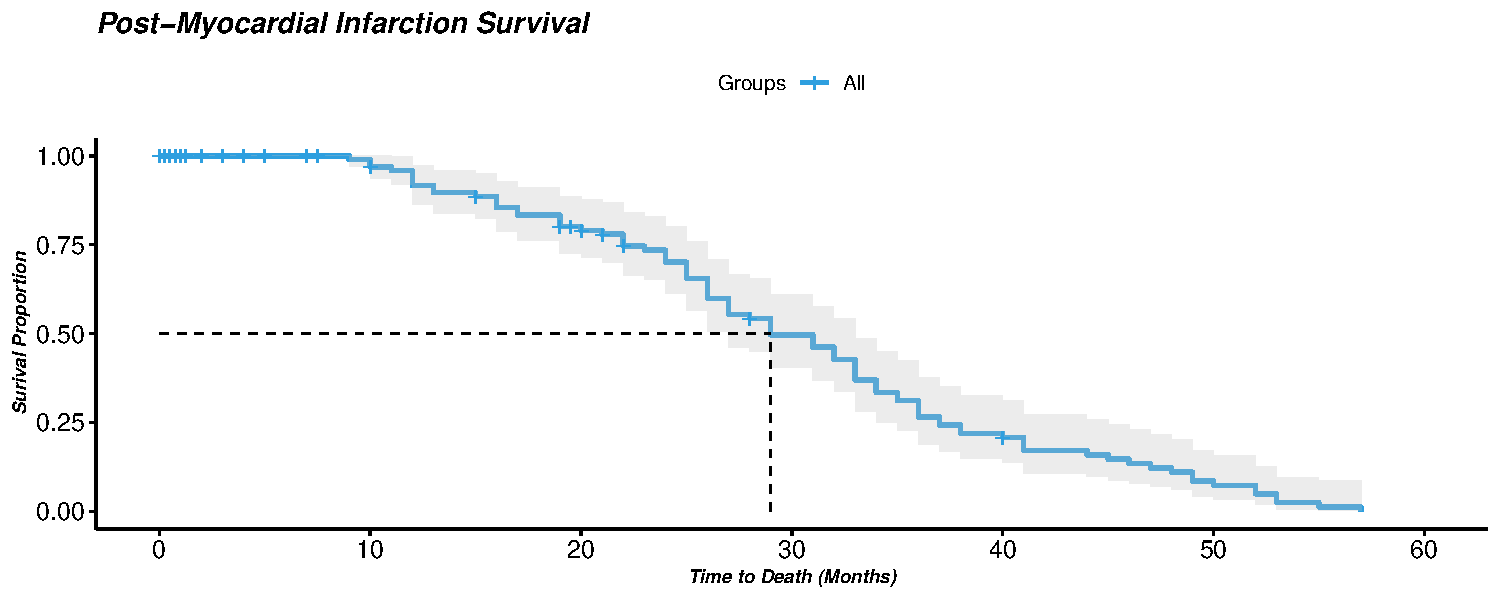
\includegraphics{markdown_files/figure-latex/km.all-1} \end{center}

Here is the survival curve for all groups within our dataset. We see
that a majority of our censored values have very short survival times.
This is primarily due to the fact that many patients joined the study
after the study began. These data points are right-censored as we do not
know their time to event. W

\begin{table}[!h]
\centering
\begin{tabular}{r|r|r|r|r|r|r|r|r}
\hline
records & n.max & n.start & events & *rmean & *se(rmean) & median & 0.95LCL & 0.95UCL\\
\hline
106 & 106 & 106 & 72 & 30.15073 & 1.23397 & 29.84 & 27 & 33\\
\hline
\end{tabular}
\end{table}

\begin{itemize}
\item
  Add stratified on age
\item
  Add stratified on cardiac physiology
\item
  Add pericardial effusion
\item
  Add median and mean + 95\% CI
\item
  Add hazard plots
\end{itemize}

\hypertarget{parametric-log-normal-model}{%
\subsection{Parametric: Log-Normal
Model}\label{parametric-log-normal-model}}

\hypertarget{parametric-log-logistic-model}{%
\subsection{Parametric: Log-Logistic
Model}\label{parametric-log-logistic-model}}

\hypertarget{parametric-weibull-model}{%
\subsection{Parametric: Weibull Model}\label{parametric-weibull-model}}

\hypertarget{cox-proportional-hazard}{%
\subsection{Cox Proportional Hazard}\label{cox-proportional-hazard}}

\hypertarget{model-diagnostics}{%
\subsection{Model Diagnostics}\label{model-diagnostics}}

\hypertarget{aic-bic-and-confidence-intervals}{%
\subsubsection{AIC, BIC, and Confidence
Intervals}\label{aic-bic-and-confidence-intervals}}

\hypertarget{residual-analysisqq-plot}{%
\subsubsection{Residual Analysis/QQ
Plot}\label{residual-analysisqq-plot}}

\hypertarget{discussion}{%
\section{Discussion}\label{discussion}}

\hypertarget{references}{%
\section{References}\label{references}}

\hypertarget{introduction-1}{%
\subsubsection{Introduction}\label{introduction-1}}

Wilmot, K. A., O'Flaherty, M., Capewell, S., Ford, E. S., \& Vaccarino,
V. (2015). Coronary Heart Disease Mortality Declines in the United
States From 1979 Through 2011CLINICAL PERSPECTIVE. Circulation, 132(11),
997--1002. doi: 10.1161/circulationaha.115.015293

Goldman, L. (1984). The Decline in Ischemic Heart Disease Mortality
Rates. Annals of Internal Medicine, 101(6), 825. doi:
10.7326/0003-4819-101-6-825

Gu K, Cowie CC, Harris MI. Diabetes and Decline in Heart Disease
Mortality in US Adults. JAMA. 1999;281(14):1291--1297.
\url{doi:10.1001/jama.281.14.1291}

Heron, M. Deaths: Leading causes for 2017 pdf icon{[}PDF -- 3 M{]}.
National Vital Statistics Reports;68(6). Accessed November 19, 2019.

Eric B. Rimm, Meir J. Stampfer, Edward Giovannucci, Alberto Ascherio,
Donna Spiegelman, Graham A. Colditz, Walter C. Willett, Body Size and
Fat Distribution as Predictors of Coronary Heart Disease among
Middle-aged and Older US Men, American Journal of Epidemiology, Volume
141, Issue 12, 15 June 1995, Pages 1117--1127,
\url{https://doi.org/10.1093/oxfordjournals.aje.a117385}

Kan, G., Visser, C., Kooler, J., \& Dunning, A. (1986). Short and long
term predictive value of wall motion score in acute myocardial
infarction. British Heart Journal, 56, 422-427.

Fryar CD, Chen T-C, Li X. Prevalence of uncontrolled risk factors for
cardiovascular disease: United States, 1999--2010 pdf
icon{[}PDF-494K{]}. NCHS data brief, no. 103. Hyattsville, MD: National
Center for Health Statistics; 2012. Accessed May 9, 2019.

\hypertarget{methodology-1}{%
\subsubsection{Methodology}\label{methodology-1}}

Tableman, M., \& Kim, J. S. (2004). Survival analysis using S: analysis
of time-to-event data. Boca Raton, Florida: Chapman \& Hall.

Salzberg, S. (1988). Exemplar-based learning: Theory and implementation
(Technical Report TR-10-88). Harvard University, Center for Research in
Computing Technology, Aiken Computation Laboratory (33 Oxford Street;
Cambridge, MA 02138).

\hypertarget{imputation-1}{%
\subsubsection{Imputation}\label{imputation-1}}

Oba S, Sato MA, Takemasa I, Monden M, Matsubara K, Ishii S. A Bayesian
missing value estimation method for gene expression profile data.
Bioinformatics. 2003;19(16):2088‐2096.
\url{doi:10.1093/bioinformatics/btg287}

Daniel J. Stekhoven, Peter Bühlmann, MissForest---non-parametric missing
value imputation for mixed-type data, Bioinformatics, Volume 28, Issue
1, 1 January 2012, Pages 112--118,

\hypertarget{discussion-1}{%
\subsubsection{Discussion}\label{discussion-1}}

Ford, E. S., \& Capewell, S. (2007). Coronary Heart Disease Mortality
Among Young Adults in the U.S. From 1980 Through 2002. Journal of the
American College of Cardiology, 50(22), 2128--2132. doi:
10.1016/j.jacc.2007.05.056

Andrikopoulos, G. K., Tzeis, S. E., Pipilis, A. G., Richter, D. J.,
Kappos, K. G., Stefanadis, C. I., \ldots{} Chimonas, E. T. (2006).
Younger age potentiates post myocardial infarction survival disadvantage
of women. International Journal of Cardiology, 108(3), 320--325. doi:
10.1016/j.ijcard.2005.05.016

Sia, Y. T., Parker, T. G., Liu, P., Tsoporis, J. N., Adam, A., \&
Rouleau, J. L. (2002). Improved post-myocardial infarction survival with
probucol in rats: Effects on left ventricular function, morphology,
cardiac oxidative stress and cytokine expression. Journal of the
American College of Cardiology, 39(1), 148--156. doi:
10.1016/s0735-1097(01)01709-0

\newpage

\hypertarget{appendix}{%
\section{Appendix}\label{appendix}}

\hypertarget{dataset-variable-summary}{%
\subsection{Dataset Variable Summary}\label{dataset-variable-summary}}

\begin{longtabu} to \linewidth {>{\raggedright}X>{\raggedright}X>{\raggedright}X}
\caption{\label{tab:Dataset.summary}Summary of Dataset Covariates}\\
\toprule
Variable & Label & Definition\\
\midrule
\endfirsthead
\caption[]{Summary of Dataset Covariates \textit{(continued)}}\\
\toprule
Variable & Label & Definition\\
\midrule
\endhead
\
\endfoot
\bottomrule
\endlastfoot
Survival & Survival & The number of months the patints survived, post-myocardial infarction.\\
\addlinespace
Status & Status & Censorship status. 0 denotes that a patient is a censored while 1 denotes that a patient is uncensored.\\
\addlinespace
Alive at the end of Survival Period & Alive.E & Binary variable. 0 denotes that patient is alive at the end of the survival period while 1 indicates that a patient is still alive.\\
\addlinespace
Patient Age & Age & The age in years when a myocardial infarction occurs.\\
\addlinespace
Age Group & Age.Strata & 0 denotes 49 or younger. 1 denotes 50 or older. 2 denotes 65 or older.\\
\addlinespace
Pericardial Effusion & P.Effusion & Binary variable. Pericardial effusion is excess fluid surrounding the heart. Though excess is not harmful, it is sometimes indicates a porly functioning heart. 0 denotes that pericardial effusion is absent while 1 denotes that fluid is present.\\
\addlinespace
Fractional Shortening & F.Shortening & Fractional shortening is a measure of contractility around the heart. Generally, lower numbers are considered to be abnormal.\\
\addlinespace
E-Point Septal Separation & EPSS & E-point septal separation is an addition measure of heart contractivity. Larger numbers are considered to be abnormal.\\
\addlinespace
Left Ventricular End-Diastolic Dimension & LVDD & Left ventricular end-diastolic dimension is the measure of the heart at the end of disatole. The larger this value is indicates a larger heart. Larger hearts are generally in poor health.\\
\addlinespace
Wall Motion Score & WMS & Wall motion score is a measure of how the segments of the left ventricle are moving during systol.\\
\addlinespace
Wall Motion Index & WMI & Wall motion index is the wall motion score divided by the number of segments that are moving. Normally, 12-13 segments can be seen in an echocardiogram.\\
\addlinespace
Wall Motion Strata & WMI.S & Binary Variable. 0 denotes that WMI is less than or equal to 1.28. 1 denotes that WMI is greater than or equal to 1.28.\\*
\end{longtabu}

\hypertarget{original-dataset}{%
\subsection{Original Dataset}\label{original-dataset}}

\begin{longtabu} to \linewidth {>{\raggedleft}X>{\raggedleft}X>{\raggedleft}X>{\raggedleft}X>{\raggedleft}X>{\raggedleft}X>{\raggedleft}X>{\raggedleft}X>{\raggedleft}X>{\raggedleft}X>{\raggedleft}X>{\raggedleft}X}
\caption{\label{tab:Dataset.actual}Original Dataset}\\
\toprule
Survival & Status & Alive.E & Age & Age.Strata & P.Effusion & F.Shortening & EPSS & LVDD & WMS & WMI & WMI.S\\
\midrule
\endfirsthead
\caption[]{Original Dataset \textit{(continued)}}\\
\toprule
Survival & Status & Alive.E & Age & Age.Strata & P.Effusion & F.Shortening & EPSS & LVDD & WMS & WMI & WMI.S\\
\midrule
\endhead
\
\endfoot
\bottomrule
\endlastfoot
11.00 & 1 & 0 & 71.00 & 2 & 0 & 0.260 & 9.000 & 4.600 & 14.00 & 1.000 & 0\\
19.00 & 1 & 0 & 72.00 & 2 & 0 & 0.380 & 6.000 & 4.100 & 14.00 & 1.700 & 1\\
16.00 & 1 & 0 & 55.00 & 1 & 0 & 0.260 & 4.000 & 3.420 & 14.00 & 1.000 & 0\\
57.00 & 1 & 0 & 60.00 & 1 & 0 & 0.253 & 12.062 & 4.603 & 16.00 & 1.450 & 1\\
19.00 & 0 & 1 & 57.00 & 1 & 0 & 0.160 & 22.000 & 5.750 & 18.00 & 2.250 & 1\\
\addlinespace
26.00 & 1 & 0 & 68.00 & 2 & 0 & 0.260 & 5.000 & 4.310 & 12.00 & 1.000 & 0\\
13.00 & 1 & 0 & 62.00 & 1 & 0 & 0.230 & 31.000 & 5.430 & 22.50 & 1.875 & 1\\
50.00 & 1 & 0 & 60.00 & 1 & 0 & 0.330 & 8.000 & 5.250 & 14.00 & 1.000 & 0\\
19.00 & 1 & 0 & 46.00 & 0 & 0 & 0.340 & 0.000 & 5.090 & 16.00 & 1.140 & 0\\
25.00 & 1 & 0 & 54.00 & 1 & 0 & 0.140 & 13.000 & 4.490 & 15.50 & 1.190 & 0\\
\addlinespace
10.00 & 0 & 1 & 77.00 & 2 & 0 & 0.130 & 16.000 & 4.230 & 18.00 & 1.800 & 1\\
52.00 & 1 & 0 & 62.00 & 1 & 1 & 0.450 & 9.000 & 3.600 & 16.00 & 1.140 & 0\\
52.00 & 1 & 0 & 73.00 & 2 & 0 & 0.330 & 6.000 & 4.000 & 14.00 & 1.000 & 0\\
44.00 & 1 & 0 & 60.00 & 1 & 0 & 0.150 & 10.000 & 3.730 & 14.00 & 1.000 & 0\\
0.50 & 0 & 1 & 62.00 & 1 & 0 & 0.120 & 23.000 & 5.800 & 11.67 & 2.330 & 1\\
\addlinespace
24.00 & 1 & 0 & 55.00 & 1 & 1 & 0.250 & 12.063 & 4.290 & 14.00 & 1.000 & 0\\
0.50 & 0 & 1 & 69.00 & 2 & 1 & 0.260 & 11.000 & 4.650 & 18.00 & 1.640 & 1\\
0.50 & 0 & 1 & 62.53 & 1 & 1 & 0.070 & 20.000 & 5.200 & 24.00 & 2.000 & 1\\
22.00 & 0 & 1 & 66.00 & 2 & 0 & 0.090 & 17.000 & 5.819 & 8.00 & 1.333 & 1\\
1.00 & 0 & 1 & 66.00 & 2 & 1 & 0.220 & 15.000 & 5.400 & 27.00 & 2.250 & 1\\
\addlinespace
0.75 & 0 & 1 & 69.00 & 2 & 0 & 0.150 & 12.000 & 5.390 & 19.50 & 1.625 & 1\\
0.75 & 0 & 1 & 85.00 & 2 & 1 & 0.180 & 19.000 & 5.460 & 13.83 & 1.380 & 1\\
0.50 & 0 & 1 & 73.00 & 2 & 0 & 0.230 & 12.733 & 6.060 & 7.50 & 1.500 & 1\\
5.00 & 0 & 1 & 71.00 & 2 & 0 & 0.170 & 0.000 & 4.650 & 8.00 & 1.000 & 0\\
48.00 & 1 & 0 & 64.00 & 1 & 0 & 0.190 & 5.900 & 3.480 & 10.00 & 1.110 & 0\\
\addlinespace
29.00 & 1 & 0 & 54.00 & 1 & 0 & 0.300 & 7.000 & 3.850 & 10.00 & 1.667 & 1\\
29.00 & 1 & 0 & 35.00 & 0 & 0 & 0.300 & 5.000 & 4.170 & 14.00 & 1.000 & 0\\
29.00 & 1 & 0 & 55.00 & 1 & 0 & NA & 7.000 & NA & 2.00 & 1.000 & 0\\
0.25 & 0 & 1 & 75.00 & 2 & 0 & NA & NA & NA & NA & 1.000 & 0\\
36.00 & 1 & 0 & 55.00 & 1 & 1 & 0.210 & 4.200 & 4.160 & 14.00 & 1.560 & 1\\
\addlinespace
1.00 & 0 & 1 & 65.00 & 2 & 0 & 0.150 & NA & 5.050 & 10.00 & 1.000 & 0\\
1.00 & 0 & 1 & 52.00 & 1 & 1 & 0.170 & 17.200 & 5.320 & 14.00 & 1.170 & 0\\
3.00 & 0 & 1 & NA & 2 & 0 & NA & 12.000 & NA & 6.00 & 3.000 & 1\\
27.00 & 1 & 0 & 47.00 & 0 & 0 & 0.400 & 5.120 & 3.100 & 12.00 & 1.000 & 0\\
35.00 & 1 & 0 & 63.00 & 1 & 0 & NA & 10.000 & NA & 14.00 & 1.170 & 0\\
\addlinespace
26.00 & 1 & 0 & 61.00 & 1 & 0 & 0.610 & 13.100 & 4.070 & 13.00 & 1.625 & 1\\
16.00 & 1 & 0 & 63.00 & 1 & 1 & NA & NA & 5.310 & 5.00 & 1.000 & 0\\
1.00 & 0 & 1 & 65.00 & 2 & 0 & 0.060 & 23.600 & NA & 21.50 & 2.150 & 1\\
19.00 & 1 & 0 & 68.00 & 2 & 0 & 0.510 & NA & 3.880 & 15.00 & 1.670 & 1\\
31.00 & 1 & 0 & 80.00 & 2 & 0 & 0.410 & 5.400 & 4.360 & NA & 1.000 & 0\\
\addlinespace
32.00 & 1 & 0 & 54.00 & 1 & 0 & 0.350 & 9.300 & 3.630 & 11.00 & 1.222 & 0\\
16.00 & 1 & 0 & 70.00 & 2 & 1 & 0.270 & 4.700 & 4.490 & 22.00 & 2.000 & 1\\
40.00 & 1 & 0 & 79.00 & 2 & 0 & 0.150 & 17.500 & 4.270 & 13.00 & 1.300 & 1\\
46.00 & 1 & 0 & 56.00 & 1 & 0 & 0.330 & NA & 3.590 & 14.00 & 1.000 & 0\\
2.00 & 0 & 1 & 67.00 & 2 & 1 & 0.440 & 9.000 & 3.960 & 17.50 & 1.450 & 1\\
\addlinespace
37.00 & 1 & 0 & 64.00 & 1 & 0 & 0.090 & NA & NA & 12.00 & 2.000 & 1\\
19.50 & 0 & 1 & 81.00 & 2 & 0 & 0.120 & NA & NA & 9.00 & 1.250 & 0\\
20.00 & 0 & 1 & 59.00 & 1 & 0 & 0.030 & 21.300 & 6.290 & 17.00 & 1.310 & 1\\
0.25 & 0 & 1 & 63.00 & 1 & 1 & NA & NA & NA & 23.00 & 2.300 & 1\\
2.00 & 0 & 1 & 56.00 & 1 & 1 & 0.040 & 14.000 & 5.000 & NA & NA & 1\\
\addlinespace
7.00 & 0 & 1 & 61.00 & 1 & 1 & 0.270 & NA & NA & 9.00 & 1.500 & 1\\
10.00 & 1 & 0 & 57.00 & 1 & 0 & 0.240 & 14.800 & 5.260 & 18.00 & 1.380 & 1\\
12.00 & 1 & 0 & 58.00 & 1 & 0 & 0.300 & 9.400 & 3.490 & 14.00 & 1.000 & 0\\
1.00 & 0 & 1 & 60.00 & 1 & 0 & 0.010 & 24.600 & 5.650 & 39.00 & 3.000 & 1\\
10.00 & 1 & 0 & 66.00 & 2 & 0 & 0.290 & 15.600 & 6.150 & 14.00 & 1.000 & 0\\
\addlinespace
45.00 & 1 & 0 & 63.00 & 1 & 0 & 0.150 & 13.000 & 4.570 & 13.00 & 1.080 & 0\\
22.00 & 1 & 0 & 57.00 & 1 & 0 & 0.130 & 18.600 & 4.370 & 12.33 & 1.370 & 1\\
53.00 & 1 & 0 & 70.00 & 2 & 0 & 0.100 & 9.800 & 5.300 & 23.00 & 2.300 & 1\\
38.00 & 1 & 0 & 68.00 & 2 & 0 & 0.290 & NA & 4.410 & 14.00 & 1.167 & 0\\
26.00 & 1 & 0 & 79.00 & 2 & 0 & 0.170 & 11.900 & 5.150 & 10.50 & 1.050 & 0\\
\addlinespace
9.00 & 1 & 0 & 73.00 & 2 & 0 & 0.120 & NA & 6.780 & 16.67 & 1.390 & 1\\
26.00 & 1 & 0 & 72.00 & 2 & 0 & 0.187 & 12.000 & 5.020 & 13.00 & 1.180 & 0\\
0.50 & 0 & 1 & 59.00 & 1 & 0 & 0.130 & 16.400 & 4.960 & 17.83 & 1.370 & 1\\
12.00 & 1 & 0 & 67.00 & 2 & 1 & 0.110 & 10.300 & 4.680 & 11.00 & 1.000 & 0\\
49.00 & 1 & 0 & 51.00 & 1 & 0 & 0.160 & 13.200 & 5.260 & 11.00 & 1.000 & 0\\
\addlinespace
0.75 & 0 & 1 & 50.00 & 1 & 0 & 0.140 & 11.400 & 4.750 & 10.00 & 2.500 & 1\\
49.00 & 1 & 0 & 70.00 & 2 & 1 & 0.250 & 9.700 & 5.570 & 5.50 & 1.100 & 0\\
47.00 & 1 & 0 & 65.00 & 2 & 0 & 0.360 & 8.800 & 5.780 & 12.00 & 1.000 & 0\\
41.00 & 1 & 0 & 78.00 & 2 & 0 & 0.060 & 16.100 & 5.620 & 13.67 & 1.367 & 1\\
0.25 & 0 & 1 & 86.00 & 2 & 0 & 0.225 & 12.200 & 5.200 & 24.00 & 2.180 & 1\\
\addlinespace
33.00 & 1 & 0 & 56.00 & 1 & 0 & 0.250 & 11.000 & 4.720 & 11.00 & 1.000 & 0\\
29.00 & 1 & 0 & 60.00 & 1 & 0 & 0.120 & 10.200 & 4.310 & 15.00 & 1.670 & 1\\
41.00 & 1 & 0 & 59.00 & 1 & 0 & 0.290 & 7.500 & 4.750 & 13.00 & 1.080 & 0\\
26.00 & 1 & 0 & 50.00 & 1 & 0 & 0.060 & 30.100 & 5.950 & 21.50 & 2.390 & 1\\
15.00 & 1 & 0 & 54.00 & 1 & 0 & 0.217 & 17.900 & 4.540 & 16.50 & 1.180 & 0\\
\addlinespace
0.25 & 0 & 1 & 68.00 & 2 & 0 & 0.220 & 21.700 & 4.850 & 15.00 & 1.150 & 0\\
0.03 & 0 & 1 & NA & 2 & 0 & 0.260 & 19.400 & 4.770 & 21.00 & 2.100 & 1\\
12.00 & 1 & 0 & 64.00 & 1 & 0 & 0.200 & 7.100 & 4.580 & 14.00 & 1.000 & 0\\
32.00 & 1 & 0 & 63.00 & 1 & 0 & 0.200 & 5.000 & 5.200 & 8.00 & 1.000 & 0\\
32.00 & 1 & 0 & 65.00 & 2 & 0 & 0.060 & 23.600 & 6.740 & 12.00 & 1.090 & 0\\
\addlinespace
27.00 & 1 & 0 & 54.00 & 1 & 1 & 0.070 & 16.800 & 4.160 & 18.00 & 1.500 & 1\\
23.00 & 1 & 0 & 62.00 & 1 & 0 & 0.250 & 6.000 & 4.480 & 11.00 & 1.000 & 0\\
0.75 & 0 & 1 & 78.00 & 2 & 0 & 0.050 & 10.000 & 4.440 & 15.00 & 1.360 & 1\\
0.75 & 0 & 1 & 61.00 & 1 & 0 & NA & NA & NA & 28.00 & 2.330 & 1\\
34.00 & 1 & 0 & 52.00 & 1 & 0 & 0.140 & 25.000 & 6.210 & 11.50 & 1.150 & 0\\
\addlinespace
1.00 & 0 & 1 & 73.00 & 2 & 0 & 0.050 & 14.800 & 4.140 & 15.50 & 1.410 & 1\\
21.00 & 0 & 1 & 70.00 & 2 & 1 & 0.160 & 19.200 & 5.250 & 11.00 & 1.000 & 0\\
55.00 & 1 & 0 & 55.00 & 1 & 0 & 0.280 & 5.500 & 4.480 & 22.00 & 1.830 & 1\\
15.00 & 0 & 1 & 60.00 & 1 & 0 & 0.180 & 8.700 & 4.560 & 13.50 & 1.040 & 0\\
0.50 & 0 & 1 & 67.00 & 2 & 0 & 0.155 & 11.300 & 5.160 & 13.00 & 1.000 & 0\\
\addlinespace
35.00 & 1 & 0 & 64.00 & 1 & 0 & 0.300 & 6.600 & 4.360 & 14.00 & 1.270 & 0\\
53.00 & 1 & 0 & 59.00 & 1 & 0 & 0.344 & 9.100 & 4.040 & 9.00 & 1.000 & 0\\
33.00 & 1 & 0 & 46.00 & 0 & 0 & 0.272 & 16.500 & 5.360 & 12.67 & 1.060 & 0\\
33.00 & 1 & 0 & 63.00 & 1 & 0 & 0.250 & 5.600 & 3.870 & 18.00 & 1.500 & 1\\
40.00 & 0 & 1 & 74.00 & 2 & 0 & 0.200 & 4.800 & 4.560 & 12.50 & 1.040 & 0\\
\addlinespace
33.00 & 1 & 0 & 59.00 & 1 & 0 & 0.500 & 9.100 & 3.420 & 18.00 & 1.500 & 1\\
5.00 & 0 & 1 & 65.00 & 2 & 1 & 0.160 & 8.500 & 5.470 & 16.00 & 1.450 & 1\\
4.00 & 0 & 1 & 58.00 & 1 & 0 & 0.170 & 28.900 & 6.730 & 26.08 & 2.010 & 1\\
31.00 & 1 & 0 & 53.00 & 1 & 0 & 0.170 & NA & 4.690 & 10.00 & 1.000 & 0\\
33.00 & 1 & 0 & 66.00 & 2 & 0 & 0.200 & NA & 4.230 & 12.00 & 1.000 & 0\\
\addlinespace
22.00 & 1 & 0 & 70.00 & 2 & 0 & 0.380 & 0.000 & 4.550 & 10.00 & 1.000 & 0\\
25.00 & 1 & 0 & 62.00 & 1 & 0 & 0.258 & 11.800 & 4.870 & 11.00 & 1.000 & 0\\
1.25 & 0 & 1 & 63.00 & 1 & 0 & 0.300 & 6.900 & 3.520 & 18.16 & 1.510 & 1\\
24.00 & 1 & 0 & 59.00 & 1 & 0 & 0.170 & 14.300 & 5.490 & 13.50 & 1.500 & 1\\
25.00 & 1 & 0 & 57.00 & 1 & 0 & 0.228 & 9.700 & 4.290 & 11.00 & 1.000 & 0\\
\addlinespace
24.00 & 1 & 0 & 57.00 & 1 & 0 & 0.036 & 7.000 & 4.120 & 13.50 & 1.230 & 0\\
0.75 & 0 & 1 & 78.00 & 2 & 0 & 0.230 & 40.000 & 6.230 & 14.00 & 1.400 & 1\\
3.00 & 0 & 1 & 62.00 & 1 & 0 & 0.260 & 7.600 & 4.420 & 14.00 & 1.000 & 0\\
27.00 & 1 & 0 & 62.00 & 1 & 0 & 0.220 & 12.100 & 3.920 & 11.00 & 1.000 & 0\\
13.00 & 1 & 0 & 66.00 & 2 & 0 & 0.240 & 13.600 & 4.380 & 22.00 & 2.200 & 1\\
\addlinespace
36.00 & 1 & 0 & 61.00 & 1 & 0 & 0.270 & 9.000 & 4.060 & 12.00 & 1.000 & 0\\
25.00 & 1 & 0 & 59.00 & 1 & 1 & 0.400 & 9.200 & 5.360 & 12.00 & 1.000 & 0\\
27.00 & 1 & 0 & 57.00 & 1 & 0 & 0.290 & 9.400 & 4.770 & 9.00 & 1.000 & 0\\
34.00 & 1 & 0 & 62.00 & 1 & 1 & 0.190 & 28.900 & 6.630 & 19.50 & 1.950 & 1\\
37.00 & 1 & 0 & NA & 2 & 0 & 0.260 & 0.000 & 4.380 & 9.00 & 1.000 & 0\\
\addlinespace
34.00 & 1 & 0 & 54.00 & 1 & 0 & 0.430 & 9.300 & 4.790 & 10.00 & 1.000 & 0\\
28.00 & 0 & 1 & 62.00 & 1 & 1 & 0.240 & 28.600 & 5.860 & 21.50 & 1.950 & 1\\
28.00 & 1 & 0 & NA & 2 & 0 & 0.230 & 19.100 & 5.490 & 12.00 & 1.200 & 0\\
17.00 & 1 & 0 & 64.00 & 1 & 0 & 0.150 & 6.600 & 4.170 & 14.00 & 1.270 & 0\\
38.00 & 1 & 0 & 57.00 & 1 & 1 & 0.120 & 0.000 & 2.320 & 16.50 & 1.375 & 1\\
\addlinespace
31.00 & 1 & 0 & 61.00 & 1 & 0 & 0.180 & 0.000 & 4.480 & 11.00 & 1.375 & 1\\
12.00 & 1 & 0 & 61.00 & 1 & 1 & 0.190 & 13.200 & 5.040 & 19.00 & 1.730 & 1\\
36.00 & 1 & 0 & 48.00 & 0 & 0 & 0.150 & 12.000 & 3.660 & 10.00 & 1.000 & 0\\
17.00 & 1 & 0 & NA & 2 & 0 & 0.090 & 6.800 & 4.960 & 13.00 & 1.080 & 0\\
21.00 & 1 & 0 & 61.00 & 1 & 0 & 0.140 & 25.500 & 5.160 & 14.00 & 1.270 & 0\\
\addlinespace
7.50 & 0 & 1 & 64.00 & 1 & 0 & 0.240 & 12.900 & 4.720 & 12.00 & 1.000 & 0\\
41.00 & 1 & 0 & 64.00 & 1 & 0 & 0.280 & 5.400 & 5.470 & 11.00 & 1.100 & 0\\
36.00 & 1 & 0 & 69.00 & 2 & 0 & 0.200 & 7.000 & 5.050 & 14.50 & 1.210 & 0\\
22.00 & 1 & 0 & 57.00 & 1 & 0 & 0.140 & 16.100 & 4.360 & 15.00 & 1.360 & 1\\
20.00 & 1 & 0 & 62.00 & 1 & 0 & 0.150 & 0.000 & 4.510 & 15.50 & 1.409 & 1\\*
\end{longtabu}

\hypertarget{imputed-dataset}{%
\subsection{Imputed Dataset}\label{imputed-dataset}}

\begin{longtabu} to \linewidth {>{\raggedleft}X>{\raggedleft}X>{\raggedleft}X>{\raggedleft}X>{\raggedleft}X>{\raggedleft}X>{\raggedleft}X>{\raggedleft}X>{\raggedleft}X>{\raggedleft}X>{\raggedleft}X>{\raggedleft}X}
\caption{\label{tab:imp.table}Imputed Dataset}\\
\toprule
Survival & Status & Alive.E & Age & Age.Strata & P.Effusion & F.Shortening & EPSS & LVDD & WMS & WMI & WMI.S\\
\midrule
\endfirsthead
\caption[]{Imputed Dataset \textit{(continued)}}\\
\toprule
Survival & Status & Alive.E & Age & Age.Strata & P.Effusion & F.Shortening & EPSS & LVDD & WMS & WMI & WMI.S\\
\midrule
\endhead
\
\endfoot
\bottomrule
\endlastfoot
11.00 & 1.00 & 0.00 & 61.86 & 1.08 & 0.18 & 0.26 & 8.22 & 4.60 & 14.00 & 1.00 & 0.00\\
19.00 & 1.00 & 0.00 & 68.39 & 2.00 & 0.25 & 0.29 & 6.00 & 4.10 & 14.52 & 1.70 & 1.00\\
16.00 & 1.00 & 0.00 & 61.82 & 1.00 & 0.00 & 0.26 & 4.00 & 3.42 & 14.00 & 1.12 & 0.00\\
22.69 & 1.00 & 0.00 & 60.00 & 1.00 & 0.00 & 0.25 & 12.06 & 4.54 & 16.00 & 1.45 & 0.95\\
19.00 & 0.00 & 0.82 & 57.00 & 1.00 & 0.26 & 0.16 & 19.69 & 5.75 & 18.00 & 2.25 & 1.00\\
\addlinespace
26.00 & 1.00 & 0.00 & 69.33 & 2.00 & 0.00 & 0.30 & 5.00 & 4.31 & 12.00 & 1.00 & 0.00\\
13.00 & 0.92 & 0.00 & 62.00 & 1.00 & 0.00 & 0.23 & 15.18 & 5.00 & 19.67 & 1.88 & 1.00\\
50.00 & 1.00 & 0.00 & 60.00 & 1.00 & 0.00 & 0.33 & 8.00 & 4.10 & 14.00 & 1.00 & 0.00\\
19.00 & 1.00 & 0.00 & 46.00 & 0.00 & 0.00 & 0.20 & 13.71 & 5.09 & 13.26 & 1.14 & 0.00\\
25.00 & 1.00 & 0.00 & 54.00 & 1.00 & 0.00 & 0.14 & 13.00 & 4.49 & 15.50 & 1.19 & 0.00\\
\addlinespace
10.00 & 0.00 & 1.00 & 77.00 & 2.00 & 0.00 & 0.13 & 16.00 & 4.23 & 18.00 & 1.80 & 1.00\\
29.84 & 1.00 & 0.01 & 62.00 & 1.00 & 1.00 & 0.24 & 9.00 & 3.60 & 16.00 & 1.14 & 0.00\\
52.00 & 0.95 & 0.00 & 73.00 & 1.70 & 0.00 & 0.33 & 6.00 & 4.00 & 14.00 & 1.00 & 0.00\\
44.00 & 1.00 & 0.00 & 60.00 & 1.02 & 0.00 & 0.15 & 10.00 & 3.73 & 14.00 & 1.00 & 0.00\\
9.11 & 0.00 & 1.00 & 59.56 & 1.00 & 0.00 & 0.14 & 23.00 & 5.80 & 11.67 & 2.33 & 1.00\\
\addlinespace
24.00 & 1.00 & 0.00 & 58.98 & 1.00 & 1.00 & 0.19 & 12.06 & 4.29 & 14.00 & 1.00 & 0.00\\
0.50 & 0.00 & 1.00 & 69.00 & 1.92 & 1.00 & 0.26 & 11.00 & 4.65 & 18.00 & 1.64 & 1.00\\
0.50 & 0.00 & 1.00 & 62.53 & 1.00 & 1.00 & 0.07 & 20.00 & 5.20 & 24.00 & 2.00 & 1.00\\
22.00 & 0.00 & 0.81 & 66.00 & 2.00 & 0.00 & 0.09 & 17.00 & 5.82 & 15.95 & 1.33 & 1.00\\
1.00 & 0.00 & 1.00 & 66.00 & 2.00 & 1.00 & 0.22 & 16.89 & 5.40 & 19.80 & 2.25 & 1.00\\
\addlinespace
0.75 & 0.04 & 1.00 & 69.34 & 2.00 & 0.00 & 0.15 & 12.00 & 5.39 & 19.50 & 1.62 & 0.96\\
0.75 & 0.00 & 1.00 & 68.54 & 2.00 & 1.00 & 0.15 & 19.00 & 5.46 & 16.32 & 1.38 & 1.00\\
0.50 & 0.00 & 1.00 & 73.00 & 2.00 & 0.00 & 0.23 & 13.91 & 5.20 & 7.50 & 1.50 & 0.79\\
5.00 & 0.00 & 0.83 & 71.40 & 2.00 & 0.00 & 0.17 & 0.00 & 4.95 & 8.00 & 1.09 & 0.00\\
48.00 & 1.00 & 0.00 & 64.00 & 1.01 & 0.00 & 0.27 & 5.90 & 3.48 & 10.00 & 1.11 & 0.00\\
\addlinespace
29.00 & 1.00 & 0.00 & 54.00 & 1.00 & 0.00 & 0.30 & 8.94 & 4.43 & 10.00 & 1.67 & 1.00\\
29.00 & 0.99 & 0.00 & 56.23 & 0.00 & 0.00 & 0.30 & 5.00 & 4.17 & 10.27 & 1.00 & 0.00\\
28.86 & 1.00 & 0.00 & 55.00 & 0.99 & 0.28 & 0.30 & 8.28 & 4.52 & 2.00 & 1.00 & 0.00\\
0.25 & 0.00 & 0.93 & 68.87 & 1.95 & 0.00 & 0.16 & 14.23 & 5.13 & 12.22 & 1.00 & 0.00\\
36.00 & 1.00 & 0.01 & 55.00 & 1.00 & 1.00 & 0.24 & 4.20 & 4.11 & 14.00 & 1.56 & 1.00\\
\addlinespace
7.61 & 0.00 & 1.00 & 65.00 & 2.00 & 0.00 & 0.15 & 12.22 & 5.05 & 10.00 & 1.00 & 0.15\\
1.00 & 0.12 & 1.00 & 52.00 & 1.00 & 0.05 & 0.13 & 17.20 & 5.32 & 14.00 & 1.32 & 0.00\\
3.00 & 0.00 & 0.99 & 68.55 & 2.00 & 0.00 & 0.12 & 12.00 & 4.97 & 20.38 & 3.00 & 1.00\\
37.79 & 1.00 & 0.00 & 47.00 & 0.00 & 0.00 & 0.40 & 5.12 & 3.10 & 12.00 & 1.00 & 0.00\\
35.00 & 1.00 & 0.00 & 59.71 & 1.00 & 0.00 & 0.21 & 10.00 & 4.27 & 14.00 & 1.08 & 0.00\\
\addlinespace
26.00 & 0.96 & 0.00 & 61.00 & 1.00 & 0.28 & 0.20 & 13.10 & 4.07 & 13.00 & 1.54 & 1.00\\
16.00 & 1.00 & 0.00 & 63.00 & 1.00 & 1.00 & 0.22 & 9.36 & 4.60 & 5.00 & 1.00 & 0.00\\
1.00 & 0.00 & 1.00 & 71.79 & 1.79 & 0.00 & 0.06 & 23.60 & 5.67 & 21.50 & 2.15 & 1.00\\
19.00 & 0.96 & 0.00 & 68.00 & 2.00 & 0.00 & 0.51 & 7.15 & 4.25 & 15.00 & 1.67 & 1.00\\
31.00 & 1.00 & 0.00 & 80.00 & 2.00 & 0.00 & 0.41 & 5.40 & 4.36 & 11.08 & 1.00 & 0.00\\
\addlinespace
32.00 & 1.00 & 0.00 & 54.00 & 0.96 & 0.00 & 0.28 & 9.30 & 3.63 & 11.00 & 1.22 & 0.00\\
16.00 & 1.00 & 0.00 & 70.00 & 2.00 & 1.00 & 0.27 & 4.70 & 4.49 & 22.00 & 2.00 & 1.00\\
26.05 & 1.00 & 0.00 & 67.70 & 2.00 & 0.18 & 0.27 & 7.70 & 4.27 & 13.00 & 1.53 & 1.00\\
46.00 & 1.00 & 0.00 & 56.00 & 1.00 & 0.03 & 0.33 & 7.89 & 4.19 & 12.06 & 1.00 & 0.00\\
2.00 & 0.00 & 1.00 & 68.25 & 2.00 & 1.00 & 0.44 & 9.00 & 3.96 & 17.50 & 1.45 & 1.00\\
\addlinespace
37.00 & 1.00 & 0.00 & 64.00 & 1.00 & 0.00 & 0.09 & 14.23 & 5.26 & 20.35 & 2.00 & 1.00\\
19.50 & 0.00 & 1.00 & 81.00 & 2.00 & 0.15 & 0.12 & 13.38 & 4.97 & 9.00 & 1.25 & 0.00\\
20.00 & 0.00 & 0.83 & 59.00 & 1.12 & 0.00 & 0.16 & 21.30 & 6.29 & 16.69 & 1.31 & 1.00\\
0.25 & 0.00 & 1.00 & 71.11 & 1.78 & 1.00 & 0.12 & 17.90 & 5.12 & 23.00 & 2.30 & 1.00\\
2.00 & 0.00 & 1.00 & 56.00 & 1.00 & 0.37 & 0.04 & 14.00 & 5.08 & 19.33 & 2.14 & 1.00\\
\addlinespace
7.00 & 0.00 & 1.00 & 61.00 & 1.00 & 1.00 & 0.16 & 11.99 & 5.00 & 9.00 & 1.50 & 1.00\\
22.69 & 0.97 & 0.00 & 57.00 & 1.00 & 0.00 & 0.24 & 14.80 & 5.26 & 14.10 & 1.38 & 0.88\\
39.57 & 0.99 & 0.00 & 58.00 & 1.00 & 0.00 & 0.30 & 7.28 & 3.49 & 14.00 & 1.00 & 0.00\\
1.00 & 0.00 & 1.00 & 60.00 & 1.00 & 0.00 & 0.01 & 24.60 & 5.65 & 39.00 & 3.00 & 1.00\\
10.00 & 1.00 & 0.00 & 66.00 & 1.79 & 0.00 & 0.17 & 15.60 & 5.07 & 14.00 & 1.00 & 0.00\\
\addlinespace
45.00 & 1.00 & 0.00 & 63.00 & 1.00 & 0.00 & 0.15 & 7.90 & 4.58 & 13.00 & 1.06 & 0.00\\
22.00 & 1.00 & 0.00 & 57.00 & 1.00 & 0.00 & 0.20 & 18.60 & 4.37 & 12.33 & 1.37 & 1.00\\
53.00 & 1.00 & 0.08 & 70.00 & 2.00 & 0.00 & 0.20 & 9.80 & 5.30 & 23.00 & 1.89 & 1.00\\
38.00 & 1.00 & 0.00 & 68.00 & 2.00 & 0.00 & 0.29 & 7.14 & 4.41 & 12.50 & 1.17 & 0.00\\
26.00 & 1.00 & 0.00 & 79.00 & 2.00 & 0.00 & 0.17 & 11.90 & 5.15 & 10.50 & 1.05 & 0.00\\
\addlinespace
9.00 & 1.00 & 0.00 & 73.00 & 2.00 & 0.00 & 0.14 & 19.43 & 6.78 & 15.17 & 1.39 & 1.00\\
26.00 & 1.00 & 0.00 & 72.00 & 2.00 & 0.00 & 0.17 & 12.00 & 5.02 & 11.45 & 1.04 & 0.00\\
4.55 & 0.04 & 1.00 & 59.00 & 1.00 & 0.00 & 0.13 & 16.40 & 4.96 & 17.83 & 1.37 & 1.00\\
12.00 & 1.00 & 0.00 & 67.00 & 2.00 & 1.00 & 0.11 & 10.30 & 4.68 & 11.00 & 1.00 & 0.00\\
27.47 & 1.00 & 0.03 & 51.00 & 1.00 & 0.00 & 0.16 & 13.20 & 5.26 & 12.11 & 1.00 & 0.00\\
\addlinespace
0.75 & 0.00 & 1.00 & 50.00 & 1.00 & 0.30 & 0.14 & 11.40 & 4.75 & 10.00 & 2.50 & 1.00\\
49.00 & 1.00 & 0.00 & 70.00 & 2.00 & 0.28 & 0.25 & 9.70 & 5.57 & 5.50 & 1.07 & 0.00\\
47.00 & 1.00 & 0.00 & 65.00 & 2.00 & 0.00 & 0.23 & 8.80 & 5.78 & 12.00 & 1.00 & 0.00\\
41.00 & 1.00 & 0.00 & 78.00 & 2.00 & 0.00 & 0.06 & 16.10 & 5.62 & 13.67 & 1.37 & 1.00\\
0.25 & 0.00 & 1.00 & 86.00 & 1.70 & 0.00 & 0.11 & 23.65 & 5.67 & 24.00 & 2.18 & 0.95\\
\addlinespace
33.00 & 1.00 & 0.00 & 56.00 & 1.00 & 0.03 & 0.25 & 11.00 & 4.50 & 11.00 & 1.00 & 0.00\\
29.00 & 1.00 & 0.00 & 59.65 & 1.05 & 0.18 & 0.12 & 10.20 & 4.31 & 15.00 & 1.67 & 1.00\\
41.00 & 1.00 & 0.00 & 59.00 & 1.00 & 0.00 & 0.29 & 8.40 & 4.75 & 13.00 & 1.08 & 0.00\\
26.00 & 1.00 & 0.12 & 60.63 & 1.00 & 0.00 & 0.06 & 16.59 & 5.18 & 21.50 & 2.39 & 1.00\\
15.00 & 1.00 & 0.00 & 54.00 & 1.00 & 0.00 & 0.22 & 17.90 & 4.54 & 16.50 & 1.18 & 0.00\\
\addlinespace
0.25 & 0.09 & 1.00 & 68.00 & 1.90 & 0.00 & 0.22 & 21.70 & 4.85 & 15.00 & 1.15 & 0.31\\
2.84 & 0.00 & 1.00 & 66.97 & 2.00 & 0.74 & 0.16 & 19.40 & 4.77 & 21.00 & 2.26 & 1.00\\
12.00 & 1.00 & 0.00 & 64.00 & 1.00 & 0.00 & 0.20 & 7.10 & 4.58 & 14.00 & 1.00 & 0.00\\
32.00 & 0.98 & 0.00 & 63.00 & 1.00 & 0.00 & 0.26 & 5.00 & 5.20 & 8.00 & 1.00 & 0.00\\
32.00 & 1.00 & 0.12 & 65.00 & 2.00 & 0.00 & 0.06 & 23.60 & 6.74 & 14.00 & 1.09 & 0.00\\
\addlinespace
27.00 & 1.00 & 0.04 & 58.49 & 1.04 & 1.00 & 0.21 & 16.80 & 4.16 & 18.00 & 1.50 & 1.00\\
23.00 & 1.00 & 0.00 & 61.34 & 1.00 & 0.00 & 0.25 & 6.00 & 4.16 & 11.00 & 1.07 & 0.03\\
0.75 & 0.00 & 0.95 & 71.49 & 2.00 & 0.00 & 0.05 & 15.08 & 5.37 & 15.00 & 1.36 & 0.96\\
3.72 & 0.01 & 1.00 & 61.00 & 1.02 & 0.00 & 0.12 & 22.80 & 5.72 & 28.00 & 2.17 & 1.00\\
34.00 & 1.00 & 0.15 & 57.09 & 1.00 & 0.00 & 0.14 & 25.00 & 5.51 & 11.50 & 1.24 & 0.00\\
\addlinespace
1.00 & 0.00 & 0.98 & 73.00 & 2.00 & 0.00 & 0.05 & 14.80 & 5.30 & 16.27 & 1.41 & 1.00\\
21.00 & 0.00 & 1.00 & 70.00 & 2.00 & 0.12 & 0.16 & 19.20 & 5.25 & 11.00 & 1.00 & 0.00\\
26.36 & 0.96 & 0.00 & 55.00 & 1.00 & 0.00 & 0.28 & 10.55 & 4.48 & 22.00 & 1.83 & 1.00\\
15.00 & 0.31 & 1.00 & 60.00 & 1.00 & 0.00 & 0.18 & 12.59 & 4.92 & 13.50 & 1.04 & 0.00\\
0.50 & 0.08 & 1.00 & 67.00 & 2.00 & 0.00 & 0.16 & 11.30 & 5.16 & 13.00 & 1.00 & 0.10\\
\addlinespace
35.00 & 1.00 & 0.01 & 64.00 & 1.00 & 0.00 & 0.30 & 6.60 & 4.36 & 12.60 & 1.27 & 0.00\\
53.00 & 1.00 & 0.00 & 59.00 & 1.00 & 0.00 & 0.34 & 7.03 & 4.04 & 9.00 & 1.00 & 0.02\\
33.00 & 0.98 & 0.00 & 46.00 & 0.00 & 0.00 & 0.22 & 16.50 & 4.64 & 12.67 & 1.20 & 0.09\\
33.00 & 1.00 & 0.00 & 60.81 & 1.02 & 0.00 & 0.25 & 5.60 & 3.87 & 14.68 & 1.50 & 0.83\\
40.00 & 0.00 & 0.63 & 74.00 & 2.00 & 0.00 & 0.20 & 4.80 & 4.56 & 12.50 & 1.04 & 0.00\\
\addlinespace
33.00 & 1.00 & 0.00 & 59.00 & 1.00 & 0.00 & 0.50 & 9.10 & 4.27 & 18.00 & 1.50 & 1.00\\
5.00 & 0.00 & 1.00 & 65.00 & 2.00 & 1.00 & 0.16 & 8.50 & 5.47 & 16.00 & 1.45 & 1.00\\
4.00 & 0.00 & 1.00 & 62.47 & 1.00 & 0.00 & 0.17 & 28.90 & 6.73 & 26.08 & 2.01 & 0.98\\
31.00 & 1.00 & 0.00 & 53.00 & 1.00 & 0.00 & 0.17 & 9.75 & 4.69 & 10.00 & 1.00 & 0.03\\
33.00 & 1.00 & 0.00 & 66.00 & 2.00 & 0.00 & 0.20 & 8.56 & 4.23 & 12.00 & 1.00 & 0.00\\
\addlinespace
22.00 & 1.00 & 0.00 & 71.44 & 2.00 & 0.00 & 0.38 & 0.00 & 4.55 & 10.00 & 1.00 & 0.00\\
25.00 & 0.99 & 0.00 & 62.00 & 1.00 & 0.07 & 0.26 & 11.80 & 4.87 & 11.00 & 1.00 & 0.00\\
21.76 & 0.00 & 0.60 & 61.57 & 1.00 & 0.00 & 0.30 & 6.90 & 3.52 & 18.16 & 1.51 & 0.83\\
24.00 & 0.96 & 0.00 & 59.00 & 1.00 & 0.00 & 0.21 & 14.30 & 5.49 & 13.50 & 1.50 & 1.00\\
25.00 & 1.00 & 0.00 & 57.00 & 1.00 & 0.00 & 0.23 & 9.70 & 4.29 & 11.00 & 1.00 & 0.03\\
\addlinespace
24.00 & 0.98 & 0.02 & 57.00 & 1.00 & 0.00 & 0.04 & 7.00 & 4.12 & 13.84 & 1.23 & 0.00\\
0.75 & 0.00 & 1.00 & 78.00 & 2.00 & 0.00 & 0.23 & 40.00 & 6.23 & 14.00 & 1.75 & 1.00\\
3.00 & 0.00 & 1.00 & 62.00 & 1.22 & 0.00 & 0.26 & 7.60 & 4.60 & 11.81 & 1.00 & 0.00\\
27.00 & 1.00 & 0.00 & 62.00 & 1.00 & 0.00 & 0.22 & 9.82 & 3.92 & 11.00 & 1.05 & 0.00\\
13.00 & 1.00 & 0.00 & 66.00 & 2.00 & 0.00 & 0.24 & 13.60 & 4.38 & 22.00 & 2.20 & 1.00\\
\addlinespace
36.00 & 1.00 & 0.00 & 58.59 & 1.00 & 0.00 & 0.27 & 9.00 & 4.39 & 12.00 & 1.00 & 0.00\\
25.00 & 1.00 & 0.00 & 59.00 & 1.00 & 0.06 & 0.40 & 9.20 & 4.36 & 12.00 & 1.00 & 0.03\\
27.00 & 1.00 & 0.00 & 57.64 & 1.00 & 0.00 & 0.29 & 9.40 & 4.77 & 9.00 & 1.00 & 0.00\\
34.00 & 1.00 & 0.00 & 62.00 & 1.00 & 1.00 & 0.19 & 28.90 & 6.63 & 19.50 & 1.95 & 1.00\\
37.00 & 0.98 & 0.03 & 69.99 & 2.00 & 0.08 & 0.27 & 0.00 & 4.38 & 9.00 & 1.00 & 0.02\\
\addlinespace
34.00 & 1.00 & 0.00 & 54.00 & 0.99 & 0.00 & 0.43 & 9.30 & 4.79 & 10.00 & 1.00 & 0.00\\
28.00 & 0.00 & 1.00 & 62.00 & 1.00 & 1.00 & 0.24 & 20.93 & 5.86 & 21.50 & 1.95 & 1.00\\
28.00 & 1.00 & 0.00 & 68.44 & 2.00 & 0.00 & 0.23 & 19.10 & 5.49 & 12.00 & 1.20 & 0.00\\
28.00 & 0.99 & 0.00 & 59.93 & 1.00 & 0.05 & 0.15 & 6.60 & 4.17 & 13.26 & 1.27 & 0.00\\
38.00 & 1.00 & 0.00 & 58.54 & 0.94 & 1.00 & 0.12 & 0.00 & 2.32 & 12.71 & 1.38 & 0.75\\
\addlinespace
31.00 & 1.00 & 0.00 & 61.00 & 1.00 & 0.00 & 0.18 & 0.00 & 4.48 & 14.82 & 1.38 & 1.00\\
12.00 & 1.00 & 0.00 & 61.00 & 1.00 & 0.10 & 0.19 & 12.28 & 5.04 & 14.59 & 1.73 & 1.00\\
36.00 & 1.00 & 0.01 & 56.98 & 0.98 & 0.24 & 0.15 & 12.00 & 3.66 & 10.98 & 1.00 & 0.00\\
17.00 & 1.00 & 0.00 & 69.20 & 2.00 & 0.00 & 0.09 & 6.80 & 4.64 & 11.76 & 1.08 & 0.00\\
21.00 & 1.00 & 0.00 & 56.76 & 1.00 & 0.00 & 0.14 & 14.00 & 5.16 & 14.00 & 1.14 & 0.00\\
\addlinespace
7.50 & 0.12 & 1.00 & 58.35 & 1.00 & 0.00 & 0.16 & 12.90 & 4.96 & 12.57 & 1.00 & 0.09\\
41.00 & 1.00 & 0.00 & 64.00 & 1.00 & 0.00 & 0.28 & 9.76 & 5.47 & 11.00 & 1.10 & 0.00\\
36.00 & 1.00 & 0.00 & 69.00 & 2.00 & 0.00 & 0.20 & 7.00 & 4.49 & 14.50 & 1.21 & 0.20\\
22.00 & 0.96 & 0.00 & 57.00 & 1.00 & 0.10 & 0.14 & 12.29 & 4.36 & 15.00 & 1.36 & 1.00\\
20.00 & 1.00 & 0.02 & 62.00 & 1.00 & 0.00 & 0.15 & 0.00 & 4.51 & 15.50 & 1.47 & 1.00\\*
\end{longtabu}

\newpage

\hypertarget{table-of-kaplan-meier-estimators}{%
\subsection{Table of Kaplan-Meier
Estimators}\label{table-of-kaplan-meier-estimators}}

\begin{table}

\caption{\label{tab:km.table}Kaplan-Meier Estimate Summary}
\centering
\begin{tabu} to \linewidth {}
\hline

\hline
\end{tabu}
\end{table}

\hypertarget{r-code}{%
\subsection{R Code}\label{r-code}}

\begin{Shaded}
\begin{Highlighting}[]
\NormalTok{knitr}\OperatorTok{::}\NormalTok{opts_chunk}\OperatorTok{$}\KeywordTok{set}\NormalTok{(}\DataTypeTok{echo =} \OtherTok{TRUE}\NormalTok{)}
\NormalTok{knitr}\OperatorTok{::}\NormalTok{opts_chunk}\OperatorTok{$}\KeywordTok{set}\NormalTok{(}\DataTypeTok{fig.height=}\FloatTok{4.5}\NormalTok{, }\DataTypeTok{fig.width=}\DecValTok{7}\NormalTok{)}

\KeywordTok{library}\NormalTok{(readxl)}
\KeywordTok{library}\NormalTok{(knitr)}
\KeywordTok{library}\NormalTok{(tidyverse)}
\KeywordTok{library}\NormalTok{(dplyr)}
\KeywordTok{library}\NormalTok{(kableExtra)}
\KeywordTok{library}\NormalTok{(survival)}
\KeywordTok{library}\NormalTok{(survminer)}
\KeywordTok{library}\NormalTok{(ggplot2)}
\KeywordTok{library}\NormalTok{(VIM)}
\KeywordTok{library}\NormalTok{(missForest)}

\NormalTok{df =}\StringTok{ }\KeywordTok{data.frame}\NormalTok{(}\KeywordTok{read_excel}\NormalTok{(}\StringTok{"df.xlsx"}\NormalTok{))}
\NormalTok{df[df}\OperatorTok{==}\StringTok{"?"}\NormalTok{] =}\StringTok{ " "}

\NormalTok{missing.data =}\StringTok{ }\KeywordTok{aggr}\NormalTok{(df) }\CommentTok{#visualize the missing information}

\KeywordTok{kable}\NormalTok{(missing.data}\OperatorTok{$}\NormalTok{missings, }\DataTypeTok{caption=}\StringTok{"Missing Values in Original Dataset"}\NormalTok{) }\OperatorTok
\StringTok{  }\KeywordTok{kable_styling}\NormalTok{(}\DataTypeTok{position =} \StringTok{"center"}\NormalTok{, }\DataTypeTok{latex_options=}\StringTok{"hold_position"}\NormalTok{)}

\NormalTok{df.m =}\StringTok{ }\KeywordTok{prodNA}\NormalTok{(df, }\DataTypeTok{noNA =} \FloatTok{0.2}\NormalTok{) }\CommentTok{#seed 10% of the missing values }
\NormalTok{df.i =}\StringTok{ }\KeywordTok{invisible}\NormalTok{(}\KeywordTok{missForest}\NormalTok{(df.m))}

\CommentTok{# dataframe rounding option}
\NormalTok{round_df <-}\StringTok{ }\ControlFlowTok{function}\NormalTok{(x, digits) \{}
  \CommentTok{# round all numeric variables}
  \CommentTok{# x: data frame }
  \CommentTok{# digits: number of digits to round}
\NormalTok{  numeric_columns <-}\StringTok{ }\KeywordTok{sapply}\NormalTok{(x, mode) }\OperatorTok{==}\StringTok{ 'numeric'}
\NormalTok{  x[numeric_columns] <-}\StringTok{  }\KeywordTok{round}\NormalTok{(x[numeric_columns], digits)}
\NormalTok{  x\}}

\NormalTok{df.new =}\StringTok{ }\KeywordTok{round_df}\NormalTok{(df.i}\OperatorTok{$}\NormalTok{ximp,}\DecValTok{2}\NormalTok{) }\CommentTok{#create the new dataset for all methods to use}
\NormalTok{s.df =}\StringTok{ }\KeywordTok{Surv}\NormalTok{(df.new}\OperatorTok{$}\NormalTok{Survival,df.new}\OperatorTok{$}\NormalTok{Status) }\CommentTok{#create the new survival obejct for all methods to use}

\NormalTok{km.all =}\StringTok{ }\KeywordTok{survfit}\NormalTok{(s.df}\OperatorTok{~}\DecValTok{1}\NormalTok{,}\DataTypeTok{type=}\StringTok{"kaplan-meier"}\NormalTok{, }\DataTypeTok{data =}\NormalTok{ df)}
\KeywordTok{ggsurvplot}\NormalTok{(km.all, }
           \DataTypeTok{palette =} \StringTok{"#2E9FDF"}\NormalTok{, }
           \DataTypeTok{conf.int =} \OtherTok{TRUE}\NormalTok{, }
           \DataTypeTok{title=}\StringTok{"Post-Myocardial Infarction Survival"}\NormalTok{, }
           \DataTypeTok{subtitle=}\StringTok{"All Groups"}\NormalTok{,}
           \DataTypeTok{font.title=}\KeywordTok{c}\NormalTok{(}\DecValTok{12}\NormalTok{,}\StringTok{"bold.italic"}\NormalTok{),}
           \DataTypeTok{font.subtitle =} \KeywordTok{c}\NormalTok{(}\DecValTok{10}\NormalTok{,}\StringTok{"italic"}\NormalTok{),}
           \DataTypeTok{font.x =} \KeywordTok{c}\NormalTok{(}\DecValTok{9}\NormalTok{, }\StringTok{"bold.italic"}\NormalTok{),}
           \DataTypeTok{font.y =} \KeywordTok{c}\NormalTok{(}\DecValTok{9}\NormalTok{, }\StringTok{"bold.italic"}\NormalTok{),}
           \DataTypeTok{ylab=}\StringTok{"Surival Proportion"}\NormalTok{, }
           \DataTypeTok{xlab=}\StringTok{"Time to Death (Months)"}\NormalTok{,}
           \DataTypeTok{surv.median.line =} \StringTok{"hv"}\NormalTok{,}
           \DataTypeTok{legend.title =} \StringTok{"Groups"}\NormalTok{,}
           \DataTypeTok{legend.labs =} \StringTok{"All"}\NormalTok{)}
\KeywordTok{kable}\NormalTok{(}\KeywordTok{t}\NormalTok{(}\KeywordTok{summary}\NormalTok{(km.all)}\OperatorTok{$}\NormalTok{table)) }\OperatorTok
\StringTok{  }\KeywordTok{kable_styling}\NormalTok{(}\DataTypeTok{position =} \StringTok{"center"}\NormalTok{, }\DataTypeTok{latex_options=}\StringTok{"hold_position"}\NormalTok{)}








\NormalTok{df.sum =}\StringTok{ }\KeywordTok{data.frame}\NormalTok{(}\KeywordTok{read_excel}\NormalTok{(}\StringTok{"df.sum.xlsx"}\NormalTok{))}

\KeywordTok{kable}\NormalTok{(df.sum, }\StringTok{"latex"}\NormalTok{, }
      \DataTypeTok{booktabs =} \OtherTok{TRUE}\NormalTok{,}
      \DataTypeTok{longtable =} \OtherTok{TRUE}\NormalTok{,}
      \DataTypeTok{linesep =} \StringTok{"}\CharTok{\textbackslash{}\textbackslash{}}\StringTok{addlinespace"}\NormalTok{,}
      \DataTypeTok{caption =} \StringTok{"Summary of Dataset Covariates"}\NormalTok{) }\OperatorTok
\StringTok{  }\KeywordTok{kable_styling}\NormalTok{(}\DataTypeTok{latex_options =} \KeywordTok{c}\NormalTok{(}\StringTok{"hold_positon"}\NormalTok{,}\StringTok{"repeat_header"}\NormalTok{),}
                \DataTypeTok{full_width =} \OtherTok{TRUE}\NormalTok{)}


\KeywordTok{kable}\NormalTok{(df, }\StringTok{"latex"}\NormalTok{, }
      \DataTypeTok{booktabs =} \OtherTok{TRUE}\NormalTok{,}
      \DataTypeTok{longtable =} \OtherTok{TRUE}\NormalTok{,}
      \DataTypeTok{caption =} \StringTok{"Original Dataset"}\NormalTok{) }\OperatorTok
\StringTok{  }\KeywordTok{kable_styling}\NormalTok{(}\DataTypeTok{latex_options =} \KeywordTok{c}\NormalTok{(}\StringTok{"hold_positon"}\NormalTok{,}\StringTok{"repeat_header"}\NormalTok{),}
                \DataTypeTok{full_width =} \OtherTok{TRUE}\NormalTok{)}

\NormalTok{round_df <-}\StringTok{ }\ControlFlowTok{function}\NormalTok{(x, digits) \{}
    \CommentTok{# round all numeric variables}
    \CommentTok{# x: data frame }
    \CommentTok{# digits: number of digits to round}
\NormalTok{    numeric_columns <-}\StringTok{ }\KeywordTok{sapply}\NormalTok{(x, mode) }\OperatorTok{==}\StringTok{ 'numeric'}
\NormalTok{    x[numeric_columns] <-}\StringTok{  }\KeywordTok{round}\NormalTok{(x[numeric_columns], digits)}
\NormalTok{    x\}}

\NormalTok{df.new =}\StringTok{ }\KeywordTok{round_df}\NormalTok{(df.i}\OperatorTok{$}\NormalTok{ximp,}\DecValTok{2}\NormalTok{)}

\KeywordTok{kable}\NormalTok{(df.new, }\StringTok{"latex"}\NormalTok{, }
      \DataTypeTok{booktabs =} \OtherTok{TRUE}\NormalTok{,}
      \DataTypeTok{longtable =} \OtherTok{TRUE}\NormalTok{,}
      \DataTypeTok{caption =} \StringTok{"Imputed Dataset"}\NormalTok{) }\OperatorTok
\StringTok{  }\KeywordTok{kable_styling}\NormalTok{(}\DataTypeTok{latex_options =} \KeywordTok{c}\NormalTok{(}\StringTok{"hold_positon"}\NormalTok{,}\StringTok{"repeat_header"}\NormalTok{),}
                \DataTypeTok{full_width =} \OtherTok{TRUE}\NormalTok{)}


\NormalTok{km.sum =}\StringTok{ }\NormalTok{km.all}\OperatorTok{$}\NormalTok{summary }

\KeywordTok{kable}\NormalTok{(km.sum, }\DataTypeTok{caption=}\StringTok{"Kaplan-Meier Estimate Summary"}\NormalTok{) }\OperatorTok
\StringTok{  }\KeywordTok{kable_styling}\NormalTok{(}\DataTypeTok{latex_options =} \KeywordTok{c}\NormalTok{(}\StringTok{"hold_positon"}\NormalTok{,}\StringTok{"repeat_header"}\NormalTok{),}
                \DataTypeTok{full_width =} \OtherTok{TRUE}\NormalTok{)}
\end{Highlighting}
\end{Shaded}

\newpage

\end{document}
